%% *************************************************************************
%%
%% This is an RIT Space Exploration Standard defining guidelines for content
%% and formatting of project design documents.
%%
%% This document uses IEEEtran.cls, the official IEEE LaTeX class
%% for authors of the Institute of Electrical and Electronics Engineers
%% (IEEE) Transactions journals and conferences.
%%
%% *************************************************************************

%% *************************************************************************
% LaTeX REFERENCES
% ----------------
%   Intro to LaTeX: http://www.rpi.edu/dept/arc/docs/latex/latex-intro.pdf
%   Comprehensive LaTeX symbol list: http://tug.ctan.org/info/symbols/comprehensive/symbols-a4.pdf
%% *************************************************************************

% tell \LaTeX what kind of formatting to use
\documentclass[conference]{IEEEtran} % http://www.ctan.org/pkg/ieeetran
% enable placeholder text generator
\usepackage{blindtext}
% enable toolbox for embedding figures and pictures
\usepackage{graphicx}
\graphicspath{ {img/} }
% enable package for adding a list of variables and constants at the beginning, aka "nomenclature"
\usepackage{nomencl}
% enable package for easily formatting units
\usepackage{siunitx}
% enable package for cross-referencing figures, sections, references etc.
% how to use hyperref: http://www2.washjeff.edu/users/rhigginbottom/latex/resources/lecture09.pdf
\usepackage{hyperref}
% change text encoding to make it more crisp
\usepackage[T1]{fontenc}
% enable conditionals for help text
\usepackage{etoolbox}

\usepackage{booktabs}
\usepackage{hyperref}
\usepackage{tabularx}

% initialize nomenclature package
\makenomenclature{}

% set title. choose something as descriptive and precise as possible. Descriptive > sounding cool. remember this!
\title{RIT Space Exploration Cube-Sat Design and Development}


\author{
  % List the authors of the design document. The Champion should go first.
  % The \$~\$ markers tell \LaTeX{} to treat the text inside to be treated as a math expression. This way you can use operators like \textcaret{} to place characters as superscripts.
  % Some \LaTeX{} templates handle the author block in different ways. For example, the \href{http://www.worldscientific.com/worldscinet/jai}{Journal of Astronomical Instrumentation} requires the authors' addresses and emails to be included as well.
  % The \textbackslash{}thanks command puts the contents inside those brackets in a footnote at the bottom of the first page. Technically speaking, \textbackslash{}thanks is just a specially formatted footnote.
  % IEEE also has a ``long form'' author block for many authors. Check here for more information:
  % \url{https://tex.stackexchange.com/questions/156523/multiple-authors-with-common-affiliations-in-ieeetran-conference-template}
  % Read here for a more advanced options to modifying footnotes in the author block:  \url{http://tex.stackexchange.com/questions/826/symbols-instead-of-numbers-as-footnote-markers}
  %   Here, we use the IEEE long-form author block.
  \IEEEauthorblockN{% This block is for author Names.
    Evan Putnam\IEEEauthorrefmark{1},
  }
  \IEEEauthorblockA{% This block is for the author Afficliations, aka department and university
    RIT Space Exploration, Rochester Institute of Technology \\ %\\ starts a new line
    Rochester, N.Y. \\
    Email:
    \IEEEauthorrefmark{1}emp9173@rit.edu,
  }
  %%   Below, we use the short-form author block and basically hack it to suit our needs.
  % Philip~Linden$^{*\dagger}$%
  %   \thanks{$^{*}$Project Champion}%
  %   \thanks{$^{\dagger}$BS/MEng '17, Mechanical Engineering},
  % Austin~Bodzas$^{\ddagger}$%
  %   \thanks{$^{\ddagger}$BS '19, Computer Science},
  % Drew~Walters$^{\S}$%
  %   \thanks{$^{\S}$BS '18, Mechanical Engineering Technology},
  % T.J.~Tarazevits$^{**}$%
  %   \thanks{$^{**}$BS '19, Game Design \& Development}%

  %%   If there are many authors, consider using symbolic, numeric (aka arabic),  alphabet footnotes or a combination thereof.
  %% the recommended order for symbolic footnotes is
  %%   (1) asterisk        *   *
  %%   (2) dagger          †   \dagger
  %%   (3) double dagger   ‡   \ddagger
  %%   (4) section symbol  §   \S
  %%   et cetera. For higher counts, use 2x symbols (1)-(4) (i.e. (5) two asterisks **). Keep cycling through (1)-(4) using 3x, 4x, and so on.
  %%   Note that these symbol codes work in math mode and text mode.
  %%   There are ways to make LaTeX do this for you, but it is more advanced and not entirely necessary, especially for short author lists. Not worth the hassle, in my opinion.
}
% page header for pages other than cover page
\markboth{Low Cost Nano-Satellite}%
{Tarazevits \MakeLowercase{\textit{et al.}}: RIT Space Exploration}

% Initial setup is over, start building the document itself
\begin{document}
\maketitle%
% correct bad hyphenation here, separated by spaces
\hyphenation{explor-ation}

\begin{abstract}
This proposal defines a multi-semester effort to design and construct RIT Space Exploration's (RIT SPEX) first Cube-Satellite, or Cube-Sat for short.  In the past SPEX has conducted a considerable ammount of research in the design of satellite and satellite sub-systems through two CSLI proposals, an investigation into the feasibility of reproducing a low cost nanosatellite from Moorehead University, as well as SMAD mission designs.  This effort is the culmination of that knowledge and the next logical step in the organizations goal of putting something into space.

      % The abstract is a brief summary of the design document. Typically it includes the purpose of the design document, key goals or objectives, and justifications.
      % Be sure not to confuse the abstract with the introduction.
      % It is easiest to write the abstract after the rest of the paper has been written.
      % That way you can choose key information from the sections that you've already completed and string them together in the abstract.
      % Consider the abstract to be your elevator pitch to anyone reading this design document.
      % What are they reading?
      % What is the goal?
      % Why is it worth my time?
      % The abstract is what will show up in Google results and other search engines, and what people will read when they are deciding what is worth their time and brain power.
\end{abstract}

\label{sec:nomenclature}
\newcommand{\nomunit}[1]{%
\renewcommand{\nomentryend}{\hspace*{\fill}#1}}
\renewcommand{\nompreamble}{
    % If you include mathematical expressions or express variables in the design document, list them with their corresponding definitions here as a list.
    % The two lines below make it look nice when defining units/values to constants.

    % Note that math terms and non-math terms are separated and alphabetized, regardless of the order in which they are defined. (Recall terms \$like this\$ are in the math environment)
    % Read more about advanced nomenclature formatting here:\\
    % \url{https://www.sharelatex.com/learn/Nomenclatures}
  }
\nomenclature{RIT}{Rochester Institute of Technology}
\nomenclature{SPEX}{RIT Space Exploration}
\nomenclature{PDD}{Project Design Document}
\nomenclature{FEA}{Finite Element Analysis}
\nomenclature{PCB}{Printed Circuit Board}
\nomenclature{CSLI}{CubeSat Launch Initiative}
\nomenclature{AMSAT}{Amateur Radio in Space}
% Below are examples of using nomenclature for math symbols and constants or units
% \nomenclature{$\dot{m}$}{Mass flow rate
%   \nomunit{\,\si{\kilo\gram\per\second}}}
% \nomenclature{$c$}{Speed of light
%  \nomunit{\,\SI{2.9979e8}{\meter\per\second}}}
\printnomenclature{}


% HELPFUL HINT: If you get the warning ``Command terminated with space.'' when using a \command try placing ``%'' or ``{}'' immediately following the command.

% The sections included here are required. Additional sections and subsections may be added as necessary.
\section{Introduction}
\label{sec:introduction}
  % The introduction is a place to give background and context before diving into the subject matter.
  % Establish context for the work you are about to propose and the main ideas of the proposition itself.

\IEEEPARstart This document outlines a three semester plan for the design and construction phase of RIT SPEX's first Cube-Sat.  RIT SPEX has had a long history with satellites and Cube-Sats and it has been a club goal for many years to build one of its own.  One of the groups earliest projects in fact was an attempt to complete a NASA Cube-Sat Launch Initiative Proposal, or CSLI.   The CSLI is a proposal where students plan, design, and construct a satellite with the partnership of NASA.  The students are responsible for everything involving design and construction where NASA approves and launches the device if they believe the benefit is appropriate.  This effort taught the group a lot about the satellite design process and the complexity of the intercommunicating sub-systems.  However, while a valuable learning experience, it was not in a state that could be submitted to NASA.  SPEX then did further research into designing its own Cube-Sat with a second CSLI.  Issues with the feasibility of the primary payload, as well as funding, proved to be too difficult to overcome in the semester timeframe.  Some other small efforts have been made to design and develop the groups first satellite but none have followed through to completion.  One such effort was the \$50 Satellite project, an attempt to replicate designs from a student group at Moorehead University.  That effort had signifigant work done in the planning stages but the technical knowledge required to fill documentation gaps was too great.
However, despite past issues and failures, it is the best time in the groups history to take on the effort of designing and constructing its first Cube-Sat.  Since the first CSLI SPEX members have worked at NASA, Lockheed Martin, Collins Aerospace, and a number of other leading aerospace companies.  Members have worked on orbital mechanics, avionics programming, and some even satellite development.  This industry experience, the clubs knowledge from previous efforts, as well as the connections students have made through these companies will help chart a path to success.




\section{Primary Objective}
\label{sec:primary-obj}
  % At the end of the day, whether the project ``succeeds'' or ``fails'' is judged against the objectives it sought to meet.
  % Note that results that contradict expectations/hypotheses are not failures if the scientific \& engineering methods are followed along the way.
  % Sometimes our expectations are wrong and that can be just as successful as getting data we thought we'd see.
  % What matters are what questions you intend to answer.
  % This is the main purpose or main goal the project hopes to achieve.

The goal is to apply members' knowledge to complete the satellite engineering development process using knowledge from the past as a springboard for development.
Members will engage in the design, fabrication, assembly and testing of space hardware and work through the unique challenges presented to construct the groups first Cube-Sat.






\section{Secondary Objectives}
\label{sec:primary-obj}
\subsection{Cube-Sat Launch Initiative}
CSLI standards and considerations should be considered and abided by.  While this project is more focused on design and construction of a satellite, the CSLI should be kept in mind for the future as the primary option for a launch.  The majority of the documentation and work done should be transferable.  This approach is different than past SPEX efforts of writing the proposal first and prolonging the start of construction.

\subsection{Reusable Architecture}
Considerations should be made for reusability in the design.  Ideally this will be the base architecture for future SPEX missions and as such software should be abstracted and component based, electrical hardware should be interchangeable, and mechanical structure should be able to support additional components.





%\begin{figure}
%  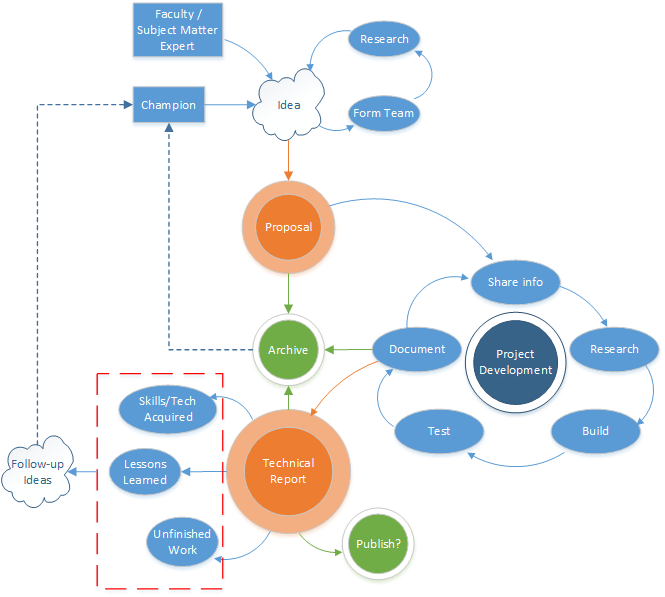
\includegraphics[width=\linewidth]{figs/project-life-cycle.png}
%  \caption{A PDD is the first piece of documentation to be archived in the project life cycle. Since the life cycle can be iterative, a new design document may also refer to one or more previous SPPs.}
%\label{fig:lifecycle}
%\end{figure}

% \section{Secondary Objectives}
% \label{sec:secondary-obj}
% Secondary Objectives are lower priority or bonus objectives that are significant but not the main focus of the project. This template does not have secondary objectives.

\section{Benefit to SPEX}
\label{sec:benefit}
% One of the core values of SPEX is to provide opportunities for academic and professional growth for its members,
% and to challenge them with interesting projects.
% In this section, explain how the project would benefit SPEX members as students,
% space enthusiasts, and young professionals.

This project will have several key benefits to SPEX in the near and long-term.
This project will create a practical astronautical engineering skillset among SPEX members, and will provide opportunities when engaging with employers to showcase the application of member skills.

% Below I have used subsections to identify key ideas in this section. These particular subsections are not required as part of the SPEX Standard, but serve as an example of using subsections in a text.

\subsection{Technical Skill Development}
\label{subsec:technicalSkills}
This multidisciplinary project will require members to learn and apply technical skills to achieve success.
Skills learned during the course of this project can be applied to many other SPEX activities as well as leveraged for future job opportunities.
The scope of this project is ideally suited for undergraduates to undergo the whole development process and gain relevant industry experience.  Some noteworthy skills or areas of knowledge that SPEX members will develop through this project include:

\begin{itemize}
\item Embedded system design
\item Digital communication knowledge
\item Fabrication
\item Project management
\item CAD
\end{itemize}


\subsection{Recognition}
\label{subsec:PublishedContent}
If this effort is successful and the device were to launch it would be the first Cube-Sat at Rochester Institute of Technology to have been to space.  There are very few groups on campus that are working on space hardware and this would increase our view on campus with the potential to solicite future funds for additional projects.  It is also noteworthy that RIT would join many other prestegious universities to have launched their own Cube-Sat.



\section{Implementation}
\label{sec:implementation}
  % What path do you anticipate the project to take?
The project will begin with payload investigations while leveraging SPEX connections for ideas.  Once a payload is chosen then the group will leverage existing resoures and Senior Design Projects to determine what can be re-used.  High level and low level requirements should then be developed for each sub-system.  Once requirements are determined parts/components must be researched and chosen for the system to begin development in an incremental approach.

\subsection{Deliverables}
\label{subsec:deliverables}
  % When all is said and done, what will you have to show for it?
  % Examples: Hardware, software, poster, ImagineRIT demo, presentations, technical papers...

The primary deliverable will be the finished, functioning Cube-Sat.
In addition, the team should have the following deliverables:
\begin{itemize}
  \item For the requirements phase of the project the group will have documentation detailing the primary payload and justification for the choice, a set of high level requirements, and detailed low level requirements.
  \item Throughout the project documentation will be maintained so it is simpler for future groups to re-implement the designs.  All documentation will be condensed and delivered at the conclusion of the project.
  \item All software written will be delivered.
  \item All CAD models/designs will be delivered.
  \item The Cube-Sat will be completed at the end of the effort and this is the primary deliverable.  Many sub-components could be considered as deliverables as well, such as communications or ADCS subsystems.
  \item Upon completion of the project a written report will be written detailing the effort.  This should be written with the intent to be become a published work.
\end{itemize}

Finally, the team will need to generate a presentation poster that could be used at ImagineRIT or other public SPEX events to highlight the project.

\subsection{Milestones}
\label{subsec:milestones}
  % Be as detailed as you can, but it's okay if there are unknowns.
  % At the very least, specify how many semester you expect the project to take until it reaches completion.

\autoref{tab:timeline} shows a preliminary timeline for the project.  In order to be effective this timeline should be maintained with minimal schedule slip.  Project management will be key to the success of the project over a three semester period, or 45 weeks.  Note that some of the phases listed can, and should, be started prior to the start of the fall semester.  In addition the it should be noted that this is very general and there may be overlap in some broad categories.  Once the team is assembled a more concrete schedule can be created.

\begin{table}
  \caption{Estimated Timeline}
  \centering
  \begin{tabularx}{\columnwidth}{@{}cXl@{}} \toprule
    Phase & Task & Duration \\ \midrule
    1 & Payload Investigations & 2 weeks or less \\
    2 & Investigation of Prior Resources & 2 weeks or less \\
    3 & Development of Requirements for each Sub-system (High/Low Level) & 1 week \\
    4 & Component Investigation & 2 weeks  \\
    5 & Development & 25 weeks  or less\\
    6 & Testing and Refinement & 10 weeks or less\\
    7 & Finalize Documentation & 1 week\\
    8 & Write Paper & 2 weeks\\ \hline
       & Total  & 45 weeks \\


    \bottomrule
  \end{tabularx}
\label{tab:timeline}
\end{table}

\subsection{Senior Design Projects}
\label{subsec:seniorDesign}
Past senior design projects have explored various areas of Cube-Sat development.  One senior design team researched solar sails and came up with a base architecture for a simple Cube-Sat.  This design will likely be taken and iterated on as our base.  It is also possible that additional senior design projects in the future will cover systems like ADCS.  It is expected that the group constructing the satellite make use of these connections and prior work done to help improve productivity and stick to schedule.

\section{Externalities}
  % Things not directly related to the work or outcomes, but related to the project as a whole.
\subsection{Prerequisite Skills}
  % Which skills do team members need to have before work can start (not including skills that will be learned ``on the job'')?
This project will likely be the most difficult thing RIT SPEX has worked on and as a result has a high barrier to entry, where likely senior members will be able to contribute the most.  The effort is multidisciplinary and will require software engineer/computer science students, mechanical engineering students, as well as electrical engineering students.  In addition it may be appropriate to have math and physics students for orbital calculations.  A number of students could also assist in the soliciation of funds for the project.

Computer Science/Software Engineer students should be familiar with C/C++ as well as object-oriented design/prototyping.  Experience with embedded systems will be very important to the success of the project as the primary avionics board will most likely be a variant of an MSP430.  

Mechanical engineers will need skills in manufacturing, thermal anaylsis, and general spacecraft design.  They will be responsible for design and analysis of all physical parts outside of the electrical system.

Electrical engineers will be the most important component to the success of the project.  These individuals will work hand in hand with the software engineers to assist in development of circuits for varying sub-systems.  Some experience with microcontrollers will be valuable to assist the software engineers to understand circuit diagrams and general electrical conecpts.  These individuals will largely be responsible for the power management system.  Electrical engineers may also contribute to the production code.


\subsection{Funding Requirements}
  % Estimate costs that would be needed to meet objectives.

This project will foreseeably be expensive.  Components in high end university or industry Cube-Sats cost thousands of dollers.  Most university estimates place their own Cube-Sats in the \$10,000 - \$100,000 range.  A signifigant portion of this cost should be from corporate and university donations in addition to the clubs own fundraising.  Signifigant cost can be reduced if some components are developed on site but that adds a reasonable level of risk to each affected sub-system.  There is possibility for a signifigant chunk, or all, of development costs to be covered under the office of the provost.

\subsection{Faculty Support}
  % Identify faculty that will be involved (or would need to be involved) to meet objectives.
  % Note that if a professor is the Principal Investigator (P.I.) for a project, there still needs to be a student as the SPEX Project Champion.
Faculty support is highly recomeneded for this project and involvement should be high.  Students should keep the faculty up to date on developments and have weekly or bi-weekly meetings to discuss work done, roadblocks, as well as any support they can give.  Ideally the faculty will take on the role of product owner while also assisting students in their respective knowledge areas.  In addition their connections with other talented students and industry leaders will be very important to the success of the project.


\subsection{Experienced SPEX Members}
Considering this project is very difficult it will require more experienced SPEX members to take part in signifigant portions of development.  The effort has been deemed a high priority item to SPEX from its faculty advisors and they  will likely ask students for assistance throughout the semester in assistance for completion of certain aspects of the project.  Due to limited number of experienced SPEX Members in certain knowledge areas, students outside of SPEX may be contacted and asked to help.

\subsection{Long-Term Vision}
\label{sec:vision}
This project would result in SPEX's first functional, space-rated hardware project.  Ideally this would result in it being put on a launch craft and being placed in low earth orbit.  In addition it will create a strong groundwork for additional satellite engineering projects.

\section*{Acknowledgements}
The author would like to thank the senior design teams that have done work for RIT SPEX in the past.  Their work on Cube-Sats has given a signifigant groundwork to start preliminary designs.

\bibliography{SPEX50SAT}


\end{document}
